% 生活与社会.tex
% Auto-generated from 感悟论语.odt by tools/odt_to_tex.py

\setpartplant{artwork/mugua.png}
  {木瓜 · 《诗·卫风·木瓜》}
  {有朋自远方来，不亦乐乎？}
  {《论语·学而》}
  {生活与社会}
\part{生活与社会}

\chapter{乱与忙}

我曾去瑞士与德国工作交换，虽然时间并不长，但却体验到了在一个安静、舒缓的环境中真正宁静而踏实地学习与研究的感觉。但回到国内后，倘若没有清醒的头脑和抵抗外界干扰的意志力，这种宁静淡泊的心态便无法萌生。然而，这并不是因为我这个人已经改变了，而仅是由于当人处在一个浮躁、纷扰的社会人文环境中，便脱离了能够滋养上述心态与生命状态的土壤，人性的弱点也更容易且多地暴露出来。

此时，提升与修炼自身固然更为重要且根本，但对于大环境的审视、反思、批判亦不可缺。毕竟，就像“年轻人就该多吃苦，吃苦才是福报”的谬论一样，在这样的大环境中磨炼一个人的性情实属残酷而无耐，是根本没有必要且原初就可以避免的。更何况，大多数人在跟环境的对抗与挣扎中获得的并非生命的提升（君子上达），而是被无情地消耗掉了宝贵的时间与精力并趋于平庸，或者在放弃与绝望中沉沦、堕落。

我想，应将造成如此局面的原因归于少数人对多数人的有意识、有目的的刻意控制。这种控制包括“乱”与“忙”两点。

\begin{itemize}
\item 乱：通过娱乐媒体、碎片化的信息或所谓知识，扰乱人的心态。同时，在“摸着石头过河”式创新与改革的进程中，不断推出朝令夕改的政策，以至于很容易使人为了适应制度并想方设法投机而惶惶不可终日。
\item 忙：通过画大饼、绘蓝图、喊口号、炒作概念、构建评价与奖励机制，使人的身体忙碌而无空暇。
\end{itemize}

因为心态无法宁静，思考便无从致远，“匹夫不可夺志”般的人生目标也就无法树立。因为忙碌，则不能在锚定个人方向后持之以恒、日积月累，从而形不成对少数人的竞争力。少数人反倒能够在乱中混水摸鱼，利用大数多人不假思索的忙碌，积累起更多的财富，更进一步地巩固其地位，并实现其自身的理想——虽然，因为往往富未必好礼、甚至为富不仁，这样的理想本身也不过是功利的、世俗的。

正因为上述潜在且无处不在的控制，令人在当下的环境中很难像在瑞士或德国那样获得真正意义上心态的放松与心情的宁静。自然地，没有了严密的思考、理性的推导、深入的研究，想要在学术上摒弃伪创新与伪首次提出，并真正有所突破就变得非常困难了。

\begin{classic}
《论语·宪问篇第十四 14.23》 子曰：「君子上达，小人下达。」

《论语·子罕篇第九 9.26》 子曰：「三军可夺帅也，匹夫不可夺志也。」

《论语·学而篇第一 1.15》 子贡曰：「贫而无谄，富而无骄，何如？」子曰：「可也，未若贫而乐，富而好礼者也。」子贡曰：「诗云：『如切如磋，如琢如磨』，其斯之谓与？」子曰：「赐也，始可与言诗已矣，告诸往而知来者。」

《论语·里仁篇第四 4.2》 子曰：「不仁者，不可以久处约，不可以长处乐。仁者安仁，知者利仁。」

《论语·里仁篇第四 4.6》 子曰：「我未见好仁者，恶不仁者。好仁者，无以尚之；恶不仁者，其为仁矣，不使不仁者加乎其身。有能一日用其力于仁矣乎？我未见力不足者。盖有之矣，我未之见也。」
\end{classic}

\entrydate{2022.09.22}

\chapter{举国体制}

“举国体制”是当下一个相当热门的讲法。例如，以举国之力发展芯片行业、造大飞机、搞大规模科研项目。似乎只要大就是好、就是了不起、就会令世人感到由衷的惊叹与敬佩。这种精神与品味倒是与电影《普罗米修斯》（Prometheus）中“工程师”（Engineers）的巨物崇拜颇为类似，是一种相对原始的、感性的冲动。

\begin{center}
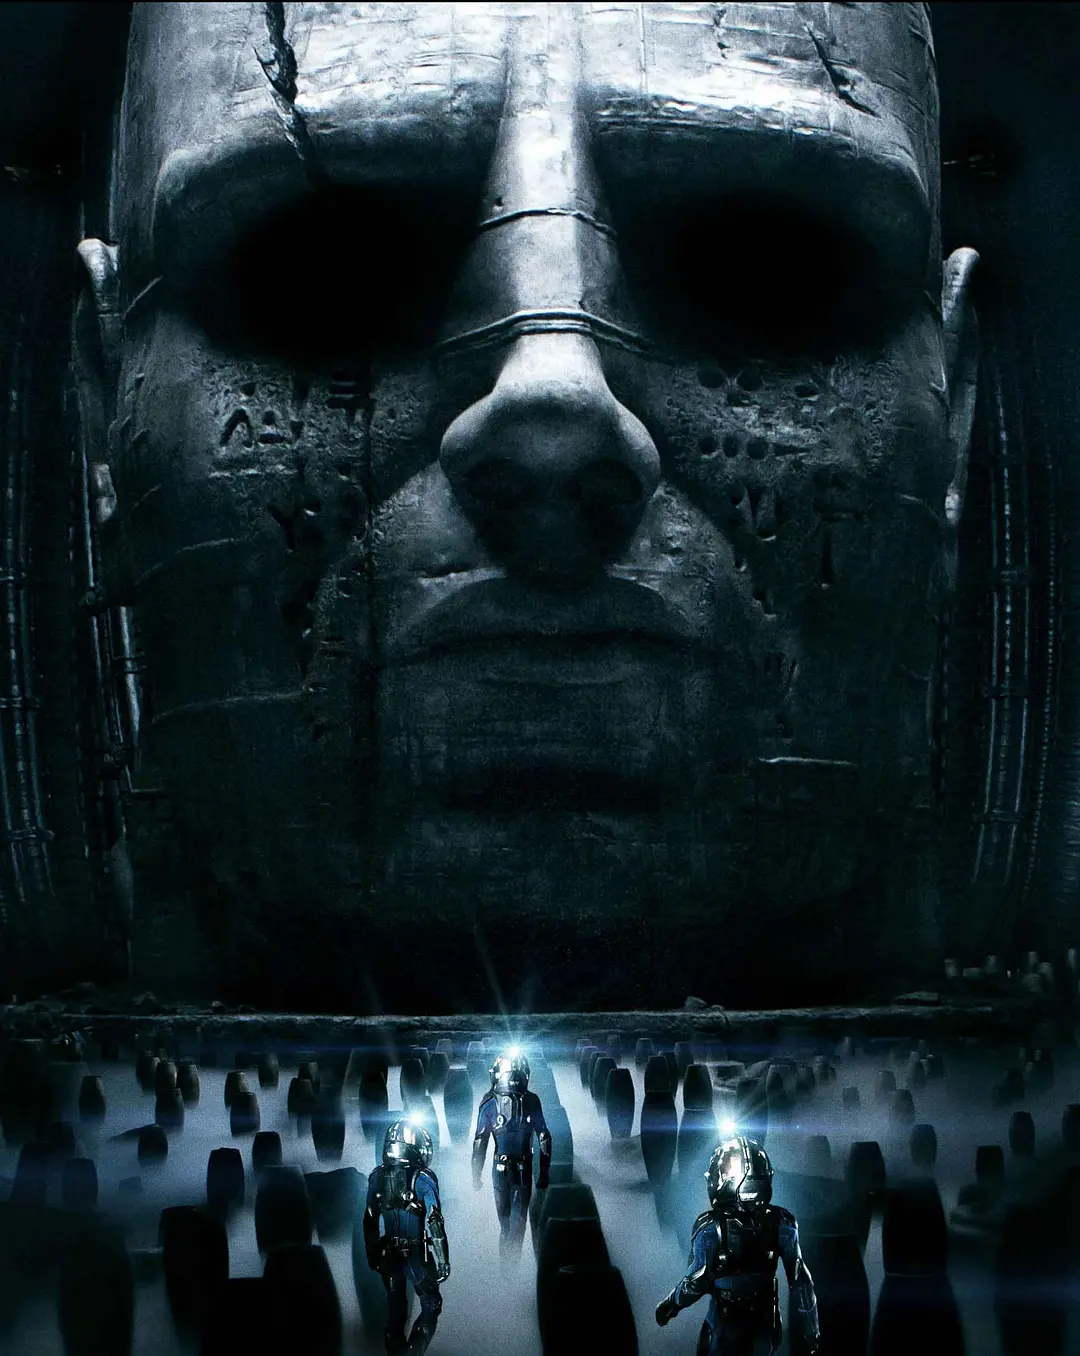
\includegraphics[width=\textwidth,height=0.62\textheight,keepaspectratio]{figures/fig02.png}
{\captiontext 电影《普罗米修斯》（Prometheus）中，当穿着宇航服、头戴头盔的探险队员们走入一座阴暗、神秘的巨大神殿时，看到了一座巨大的石雕人脸，这是“工程师”文明的遗迹。\par}
\end{center}

基于 \textbf{现成} 的科学知识、技术、工具并加以运用，“举国体制”虽然非常适合修筑长城与金字塔这样的 \textbf{大工程} ，但却无法孕育毕达哥拉斯、苏格拉底、牛顿、康德、高斯这类引领人类不断提升的伟大哲人与科学家，也不适合基础性、真创新性的学科，因此绝非万能药（panacea）。这是由于举国体制自身的工程性、实用性、功利性、运动性使其无法应对来自纯粹理性的普遍性与必然性的降维打击。

具体到个人，举国体制无法替代以真善美作为哲思与科研的终极目标而产生出的强大而持久的自驱力，以及在此目标指引下持续积累、反复练习、不断打磨出的小而美、小而精的优雅品质。在热火朝天的大干、快干中，个人的精力与潜力很容易被浪费、消耗，在激情中也难以维持宁静的心态并将理性与智慧发挥到极致。

另一方面，我们理性的运作与对于真理、真知的追求有其自身的规律与节奏，不可能永远与所谓的举国体制合拍，也不应当一直主动迎合。我们在自己研究方向上的科学探索、达成理解与完善技艺是一生一世的大事业，而举国体制所能支撑的某个方向与行业的热点大项目充其量也就不过十年。过度地适应与迎合，就会使自己陷入一会儿顺风顺水符合国家大趋势，一会儿又被体制与评价机制淘汰出局的量子迭加态。人生短暂，该拿什么作为我们人生与事业的核心来一以贯之，是每个人需要深刻思考与具体实践的大问题。

更进一步讲，总有一些根本的、绝对的、极度困难的学术与技术问题，就算没有国家的补贴、政策的支持、资本的助推、他人的认可，我们也一定要亲自去研究、摸索一番，乃至要把所有的死胡同都走过几遍之后，才能最终杀出一条血路。而这就是科研的第一推动力，也是“克己复礼”、“匹夫不可夺志”、“我欲仁，斯仁至矣”儒家精神的体现。引用阿德勒的话：“必须有人开始。即使别人不合作，那也与你无关。我的意见就是这样。应该由你开始，不用去考虑别人是否合作。”

\begin{classic}
《论语·卫灵公篇第十五 15.3》 子曰：「赐也，女以予为多学而识之者与？」对曰：「然，非与？」曰：「非也！予一以贯之。」

《论语·颜渊篇第十二 12.1》 颜渊问仁。子曰：「克己复礼，为仁。一日克己复礼，天下归仁焉。为仁由己，而由仁乎哉？」颜渊曰：「请问其目？」子曰：「非礼勿视，非礼勿听，非礼勿言，非礼勿动。」颜渊曰：「回虽不敏，请事斯语矣！」

《论语·子罕篇第九 9.26》 子曰：「三军可夺帅也，匹夫不可夺志也。」

《论语·述而篇第七 7.30》 子曰：「仁远乎哉？我欲仁，斯仁至矣。」
\end{classic}

\entrydate{2022.10.08}

\chapter{有教无类}

\begin{classic}
《论语·卫灵公篇第十五 15.39》 子曰：「有教无类。」

《论语·述而篇第七 7.22》子曰：「三人行，必有我师焉：择其善者而从之，其不善者而改之。」
\end{classic}

看到姜萍这样的人脱颖而出，且无论最终的比赛结果怎样、事件的真伪有无戏剧性反转，对于独立从事数学算法研究与开发、很多时候孤立无援的我来说，已着实是非常振奋人心了。

无论是出于平庸人内心的嫉妒，还是出于好奇心追求所谓的真相，质疑者虽无可厚非，但就像只为了获胜而辩论的辩手无法从争论中获得深层次的理解、共鸣与启迪，他们也无法从此人此事获得鼓舞与激励，从而有助于自我提升。孔子说的“攻乎异端，斯害也已”正是这个道理。当一个人内心对谁也不服气，对任何比他（无论是表面上还是实质上）优秀的人的第一反应都是抱以怀疑，这难道不是自大的表现么？人应当有对他人的卓越心悦诚服，并借机改进自己行动与习惯的意愿、能力和行动力。

鉴别姜萍有没有真才实学非常简单，只要有一个教授“屈尊”和姜萍面谈一次就水落石出了。但目前尚未看到有谁这么做。想来这已不是有没有伯乐的问题，而是连基本的任人唯贤、任人唯才都做不到。

事实上，姜萍发展的好坏与否毕竟与官员、教授的私利无关，甚至还可能对现有的高考制度、教育与学术体系产生解构的作用——因为当大众发现真才实学、学术自由、真正的创新与突破可以无需借助赢利性和世俗化的教育体系来外求，而终究只能靠个人求索来实现的时候，一直以来垄断学术资源与话语权的教育体系的权威性与光环便会削弱了。这样看来，没有哪个学校或专家愿意站出来打破惯例或做“出格”的事情也便很自然了。更何况，想要那个决定多少代人一生命运的机械的高考制度具有灵活性，本来也不是件容易的事。其前提是人心尚未堕落，且仍怀有理想与纯真，体制自身没有那么多腐败。以这个标准来看，中国还不具备这个条件。

无论是从微观的个人能否心怀敬佩的角度出发，还是从宏观体制是否清明、灵活的角度出发，反思大约一百年前英国皇家学会的数学家哈代发现、帮助拉马努金并与之合作结出硕果的感人事迹，才会发现要想践行与实现“伯乐”之难。同时，由“伯乐”这一典故也可略见我们的一大症结，即讲话与写作中的用词、造句都很漂亮，引据经典（非理论、理性的经典）亦看似博学，但是否真正能够做到以及做到了什么程度，则距离真善美的极至，或者退一步讲，距离人类历史已达到的高度相去甚远。但不管怎样，在现实与理想中，我们都需要有哈代与拉马努金。

\entrydate{2024.06.18}

\chapter{新年随想与寄语}

新年伊始往往是人们系统化回首过去和展望未来的好时机。就像不知是谁在这个新旧交替之际设置了一个颇具特殊意义的时间节点，正好适合品尝收获的甜美果实，并将行囊重新填满以信心和希望。

然而，“子在川上曰：逝者如斯夫”！时间本是如同河流，它相对于人短暂的一生来说，没有终始，更无预先划定的阶段与界限。虽然，因为每天的日出日落一直以来影响着人的作息，以“天”为单位的“日叁省吾身”是自然而合理的；然而所谓的“年”，便不过是地球绕太阳公转的周期。若以之作为人类生活的中、长期节律，在古代人类被庄稼“驯养”的农业社会倒还有一定的合理性，但到了如今工业化与信息化的经济时代，则只能是纯粹人为的设定，以至于既不具有时空绝对意义，也不具有个人生活与社会活动的现实意义了。

其实，两千多年前的孔夫子似乎也并无有关新年寄语或随想的只言片语。除了上文提到的把河流比作时间外，只闻他说过“君子无终食之间违仁”。对于谨小慎微的曾子，则是“如履薄冰”般地“日叁省吾身”。这样看来，我们的回顾、反省、规划、展望应当立体化地在短期、中期、长期多个维度上时时进行。每一分、每一秒以及做出的每一个选择均是极为重要的。与此同时，人的生命历程恰如一次无比漫长的星际旅行。立下的目标应当是一生的，从事的事业也是一生的。在这一生的求索历程中，每个人的人生有其自己的内在韵律和本征模式。而那些有待探索和发现的里程碑，也绝不会受到“年”的限制。

总之，新年之际的规划与展望其实已不再有什么特殊的意义，也更不应该成为一年中仅有的一次系统化自我整理的契机。由此送上我的2018新年寄语：

跳出时空的维度去了解你自己吧！发现你内在的人生韵律和本征模式！从现在开始，努力定位到属于你自己的那颗遥远的明星，开启一次精彩、历险且永不回头的星际航行！

\begin{classic}
《论语·子罕篇第九 9.17》 子在川上曰：「逝者如斯夫！不舍昼夜。」

《论语·里仁篇第四 4.5》 子曰：「富与贵，是人之所欲也，不以其道得之，不处也。贫与贱，是人之恶也，不以其道得之，不去也。君子去仁，恶乎成名。君子无终食之间违仁，造次必于是，颠沛必于是。」

《论语·泰伯篇第八 8.3》 曾子有疾，召门弟子曰：「启予足！启予手！诗云：『战战兢兢，如临深渊，如履薄冰。』而今而后，吾知免夫！小子！」

《论语·学而篇第一 1.4》 曾子曰：「吾日三省吾身，为人谋而不忠乎？与朋友交而不信乎？传不习乎？」
\end{classic}

\entrydate{2018.01.01}

\chapter{有朋自远方来}

《The Man Who Knew Infinity》书中提到Littlewood与Hardy的交往：

\begin{classic}
Littlewood had recently moved into rooms on D Staircase of Nevile’s Court. Pausing in the arched doorway at the staircase’s base, he could sight through the portico to the arches across the court framed within it. It was an arresting view—perhaps one reason he remained there for sixty-five years, until his death in 1977. From Hardy’s rooms, it was just nineteen steps down the winding stone staircase, then forty paces through the gate into Nevile’s Court and around to D Staircase. Yet normally the two men communicated by mail or college messenger and did not, in any case, routinely run off to confer with one another in person. And so, that winter evening in 1913, to let Littlewood know he wished to meet with him after Hall, Hardy sent word by messenger.
\end{classic}

二人的办公室虽然仅仅相距十九级台阶再加四十步，他们之间的交流却仍大多通过信件与信使，而不经常面谈。然而，这丝毫不妨碍他们之间的密切合作与深刻思想的碰撞交流。想来这就是我们常说但却鲜见的“君子之交”吧！而其中蕴含的精神与孔子和蘧伯玉的交往有着异曲同工之妙。

\begin{classic}
《论语·宪问篇第十四 14.25》 蘧伯玉使人于孔子，孔子与之坐而问焉。曰：「夫子何为？」对曰：「夫子欲寡其过而未能也。」使者出。子曰：「使乎！使乎！」
\end{classic}

可以看出，君子专注于“务本”，执著于对真善美的追求。因为“无终食之间违仁”，须臾不能离道，所以实再是没有功夫用来宴乐、交际。 这样一来，有限却深入的交流便显得弥足珍贵，偶尔的造访则更是成为铭记于心的乐事。然而，这样的朋友能否寻得，既须以自身的好学与修行为基础，也要看缘分。如有，则实属上天眷顾；没有，则仍需独自砥砺前行。

\begin{classic}
《论语·学而篇第一 1.2》 有子曰：「其为人也孝弟，而好犯上者，鲜矣；不好犯上，而好作乱者，未之有也。君子务本，本立而道生。 孝弟也者，其为仁之本与！」

《论语·里仁篇第四 4.5》 子曰：「富与贵，是人之所欲也，不以其道得之，不处也。贫与贱，是人之恶也，不以其道得之，不去也。君子去仁，恶乎成名。君子无终食之间违仁，造次必于是，颠沛必于是。」

《论语·季氏篇第十六 16.5》 孔子曰：「益者三乐，损者三乐。乐节礼乐，乐道人之善，乐多贤友，益矣。乐骄乐，乐佚游，乐宴乐，损矣。」

《论语·卫灵公篇第十五 15.17》 子曰：「群居终日，言不及义，好行小慧，难矣哉！」

《论语·学而篇第一 1.1》 子曰：「学而时习之，不亦说乎？有朋自远方来，不亦乐乎？人不知而不愠，不亦君子乎？」

《论语·子罕篇第九 9.30》 子曰：「可与共学，未可与适道；可与适道，未可与立；可与立，未可与权。」
\end{classic}

\entrydate{2022.03.14}

\chapter{道不同，不相为谋}

子曰：「道不同，不相为谋。」两个人即便在做同一个方向的研究，从事同一个领域的事业，因为各自有不同的终极目标、价值判准、做事风格、处世之道，想要达成一致根本不大可能，能寻得大体上的理解与认同就已实属不易了。人的一生虽然漫长，但十有八九遇到的也就是这么个情况。应对此局面的最佳态度倒也同样出自论语，即“刚毅木讷”。

所谓“木讷”，是出于两个人完全处在不同的频道上，难以相互理解并达成理想的一致，所以过多的讲述与解释也无非是浪费时间，甚至自取其辱。而之所以要做到“刚毅”，则是我们在不奢求有志同道合者的情况下，仍旧能够守得住原则，耐得住寂寞，既不会人云亦云，更不会借热门炒作。唯一要做的就是勤勉学习，敏于做事，闻道日肥。这难道不正是达成目标最高效的途径么？

\begin{classic}
《论语·宪问篇第十四 14.29》 子贡方人。子曰：「赐也，贤乎哉？夫我则不暇！」

《论语·卫灵公篇第十五 15.40》 子曰：「道不同，不相为谋。」

《论语·子罕篇第九 9.30》 子曰：「可与共学，未可与适道；可与适道，未可与立；可与立；未可与权。」
\end{classic}

\entrydate{2023.01.08}

\chapter{致友人的一封信}

以下截选自我曾写给友人的一封信。希望能在那些（尤其是走出学校后）一直坚持学术精神、热爱与追求技术的朋友心中产生一些共鸣。

很高兴看到你的心境得到改观，更平静地看待以前的人与事。人生总有些许无耐，每个人生均属不易——所以才需更加宽容！你若看过《永恒的爱》（Immortal Beloved）这部演艺贝多芬情感经历的电影，你会觉得我们要幸运得多。

根据你的描述，你目前的工作职位虽然号称是研究型，但每天实质上做的基本为重复性工作，而且还要在较短的周期内应对和解决诸多客户的问题。如此一来，工作不紧张才怪，不无聊才怪！其实，这也就是你的部门经理对你职位的定位，以及公司高层对你们部门工作性质的定位吧！再想想看，我们自己的出发点和立场何时与领导者的意愿真正是一致呢？他们考虑的是如何向上级交出成果，要快、要多，甚至可以因此忽略质量，无视技术；而我们自己则是希望所做的事情有技术价值和学术意义，并且能够怀有兴趣与热情去做自己渴望的研究工作，从而实现个人的发展以及对公司和社会的价值。可以看出，我们不过是一个被公司调用的棋子，有相当的时间可能不是为了技术本身而是为了一个无理头的决定或者是他人的颜面工作，谁又会考虑你个人的技术发展呢？所以，自己的路子还是要自己选择，自己来走，且应不断地调整。除非你真的到了很高的境界变得有话语权和影响力，这种调整的过程不会停止。

《大学》有云：

\begin{classic}
大学之道，在明明德，在亲民，在止于至善。知止而后有定，定而后能静，静而后能安，安而后能虑，虑而后能得。物有本末，事有终始，知所先后，则近道矣。
\end{classic}

《大学》章句为古之学者初学入门必读。由上面所摘首句即可看出，学者第一要务为明确自己的终极追求，即至善之地。若于为学伊始即立下此志，整个人生便会有所定向，才能做到心静如水，而宁静方能致远。对于我们来说，从走入科研大门的那一天开始，恐怕这样的立志就是颇为模糊的，甚于是缺失的。于是，在后续的研究与工作中，因为不明确自己“一定要做什么”以及“一定不能做什么”（后者尤为重要，它决定了你的底线），以至于从表面上看来我们做了一大堆项目，但却失去了对技术的专注与专业度，学术的素质与品味亦毫不见长 。长此以往，你就会发现离自己的初衷与梦想越来越远，可眼下的能力却又不足以说服他人支持你做想往的事情。这种理想与现实，理想与个人实力间的落差会让人陷入痛苦的泥淖。

想要从这样的泥淖中解脱确不是一件易事。毕竟，一个人在他现有的档次甚至是降级以做得风声水起乃至获得丰厚的利益是相对容易的。而要想让已成为社会人、成为为他人服务工具的自己再进阶一个层次则要付出百倍的努力。但无论怎样，你需要首先做到：始终不忘思忖自己的至善之地究竟在何处？其实，答案也许并不难得出：当你每每对于现状不满、失望，以至于情绪低落、琢磨着该怎么改变的时候，恰恰是上天向你暗示何处是属于你的至善之地的时候。只不过，由于我们已经习惯于目前的生活与工作环境，习惯于每天上下班的节奏与沿途的景致，以至于不愿意或者害怕有所改变——这就是积习的力量，也是懒惰的力量。其实，精神上的痛苦还不足以告诉我们自己真正想做的事吗？至少，这还不足以告诉我们哪些是自己不愿做的事吗？

有了终极目标，心即可归于安定与宁静。此时，即便是工作与生活还在变动，仍令人不满意，但心已不会随之纷乱。开始时，只能利用业余时间不断积累， 待时机成熟，则可全身心投入。统计一下：如果每天都能在一个方向上坚持积累2\textasciitilde{}3小时，经过8年即可达到10000小时。据网上的说法，此时就可以成为该领域的专家了。况且，由于我们对于原本想往的领域并非一窍不通，实际达成目标的时间可能还要更短。我想，这一点对于你也是适用的吧！

\entrydate{2016.12.04}

\chapter{断电小记}

前天晚上屋里突然断电。最先以为是入户电表跳闸——因为前一阵出现过同样的问题——然而，查看后才发现是屋内厨房地插的总闸跳掉了。于是，第二天跟物业预约了电工师傅上门检修。晚上六点半多，来了一位二十多岁的小伙子，我便开始和他一起在没有空调与风扇的闷热环境下忙到了八点半左右。其间，我们将厨房里所有的电源插座都拆开排查了一遍。他还穿过草丛，跳到小院里，寻找是否有从屋里引出到外面的插座。可结果，除了发现电气布线是一团糟外，根本没有可以快速解决的办法。看到小伙子浑身被汗水浸透，我的心里颇为过意不去。虽然问题并未得到解决，也没有更换任何部件，我仍旧给他微信转了维修费，从而稍感安慰。待小伙子走后，我顾不上吃饭，立即着手重新布置多个插排。到晚上十点钟，便将卫生间的电引出到了厨房，从而生活电器得以恢复使用U+3002至此，心里才觉得踏实，吃了点面包和水果当作夜宵。

可见，生活中总会遇到不如意的事。对此，应当以乐观的态度积极面对，将其看作是对自身的考验与磨炼。从而让自己像是沙漠中的红柳，总能够从困难与逆境中汲取有益的养分。同时，维修小伙子不怕脏、不怕苦的敬业精神也值得我虚心学习，并将这种精神迁移到数学研究上。

\begin{classic}
《论语·子罕篇第九 9.14》 子欲居九夷。或曰：「陋，如之何？」子曰：「君子居之，何陋之有！」

《史记·孔子世家第十七》 孔子曰：“回，诗云“匪兕匪虎，率彼旷野”。吾道非邪？吾何为於此？”
\end{classic}

\entrydate{2019.07.20}

\chapter{攻乎异端，斯害也已}

从网上看到一则消息，某人因为撰写了一篇药酒具有毒性的文章，而被派出所缉拿后关押了数月，后获得保释。若只是以此消息作为情景剧的素材而不追究事实真相，通过做一些虚拟假设来看看能否从中推导出为我们受用的结论，那么倒不妨将该事件设想为此人凭藉科学知识向奸商发起质疑和抨击，结果反倒因为商警勾结而含冤入狱。

基于这样的情景假设，我们便可以学到一点：最好通过做正确、积极、高尚的功业来吸引、影响和引导人，从而自然地令低劣产品难有市场生存空间，使污秽、恶劣的行径无藏匿之处；而不宜以举报、接发为己任，做针锋相对的事情，以至于在双方消耗的过程中虽然对恶势力也形成了一定的打击，但是良性的事业也没有因此得到培育和发展的机会。这种看似没有硝烟的斗争其实也是儒家智慧的体现，因为孔子有云：

\begin{classic}
《论语·为政篇第二 2.16》 子曰：「攻乎异端，斯害也己。」
\end{classic}

试想，孔子在春秋礼崩乐坏的时期，也并没有四处抨击当政者，更没有操戈厮杀于战场，而是用宣传礼乐教化的方式，培养了一大批人，在时间与地域的广大尺度上产生了深远的影响。世间的恶势力仅凭一个人、一群人、甚至一代人是无法肃清的，至多是拔除一些毒草，但仍无法撼动根基，更难以给人心、人性带来潜移默化的影响。所以更好的方式就是靠个人的积累、修炼、实践来起到“己欲立而立人”般的示范作用。之所以人心尚存很多恶，原因之一便是在这个“烂透了”的世界上，要做成一件从初衷开始，并从头至尾没有欺骗和原罪的正确的事业着实是“too damn hard”。人们因鲜见到有品味的成功案例与“以其道得之”的富贵，以至于失去信心，放弃甚至毁坏了人性向善的本质。

既然事已至此，我们就应当做出笃实而正确且完全合乎义的事业来向世界展示什么是真、善、美；要以此告诉世人我们每个人原本完全可以不必扭曲、憋屈、丧失自我地过活，也完全可以且应当享受和欣赏到货真价实、有质量、有品味、有美感的事物。即便终其一生也未能完成这样的事业，相信也会有志同道合者的接力。如此形成良性循环，善莫大焉。

\entrydate{2018.09.28}

\chapter{疫情之下《论语》带给我们的启示（一）}

新冠疫情的肆虐令 2020 年成为整个人类历史上极其不平凡的一年。直至今日，我们仍难以准确预期人类彻底战胜疫情的那一天。在这段艰难的岁月里，我们依然可以从《论语》中汲取着营养，将其渗透到生活的点滴之中。在《论语·公冶长》一篇中，孔子将他的志向总结为“老者安之，朋友信之，少者怀之”。曾子也说过“慎终追远，民德归厚矣”。这就教导我们对每一个具体的生命无分男女老幼，均应无比敬重和珍视。

\begin{classic}
《论语·公冶长篇第五 5.26》 颜渊、季路侍。子曰：“盍各言尔志？”子路曰：“愿车马、衣轻裘，与朋友共，敝之而无憾。”颜渊曰：“愿无伐善，无施劳。”子路曰：“愿闻子之志。”子曰：“老者安之，朋友信之，少者怀之。”

《论语·学而篇第一 1.9》 曾子曰：“慎终追远，民德归厚矣。”
\end{classic}

从《论语》中我们还可以看到，孔子所慎重的三件事中，“疾病”便占了其中一端。

\begin{classic}
《论语·述而篇第七 7.13》 子之所慎：齐，战，疾。
\end{classic}

这是因为，生命的安全与身体的健康是一个人得以持续行仁，在成为君子、止于至善的道路上坚持学习、慎思笃行、不断提升，并为国家与社会贡献价值的大前提。所以，我们必须予以高度的重视。这个时候，要了解、相信科学，以科学事实为依据，不要妄信和转发网上不靠谱的防疫或治病偏方。对此，《论语·乡党篇第十 10.16》也记载到，

\begin{classic}
康子馈药，拜而受之，曰：“丘未达，不敢尝。”
\end{classic}

孔子说过“危邦不入，乱邦不居”。所以，当下我们要尽一切可能避免去高危地区，尤其是社会动荡与政治混乱的国外。最好的做法就是待在自己当前生活与工作的地方，甚至是深居简出，自行居家隔离。这既是关照个人的健康，也是为他人和整个社会的生命安全负责。当然，在固守一地的日子里，生活未免有些单调。然而，只有“不仁者，不可以久处约”。只要我们以“行仁”作为精神核心，约束我们的言语、限制出行范围，反倒能够利用这段时间做一些深入、长远的思考，开展系统、专注的学习，好好修炼思想、端正态度、完善知识、提升技能。

\begin{classic}
《论语·泰伯篇第八 8.13》 子曰：“笃信好学，守死善道。危邦不入，乱邦不居，天下有道则见，无道则隐。邦有道，贫且贱焉，耻也，邦无道，富且贵焉，耻也。”

《论语·里仁篇第四 4.2》 子曰：“不仁者，不可以久处约，不可以长处乐。仁者安仁，知者利仁。”
\end{classic}

若我们与父母在不同的地方居住生活，则要尽量让彼此的距离不要相隔太远，从而无论疫情有何突发的状况，都能够相对方便地彼此相互照应、扶持。如果我们实在没有办法做到“不远游”，则应与父母保持比平时更加频繁的联系，随时报平安，让父母放心。

\begin{classic}
《论语·里仁篇第四 4.19》 子曰：“父母在，不远游，游必有方。”
\end{classic}

疫情之下，经济萧条、就业形势亦不乐观，这很容易让我们产生强烈的危机感和对未来职业发展的迷茫。这里，《论语》对我们的教导则是“人无远虑、必有近忧”。所以，我们应当具备长远的眼光，围绕核心技术、基础理论持续发力、做足准备，最终一定能从危机中发现社会发展的必然趋势、找到蕴藏于其中能够自我实现、服务国家的机会。

\begin{classic}
《论语·卫灵公篇第十五 15.12》 子曰：“人无远虑，必有近忧。”
\end{classic}

总之，只要我们在这段特殊的时期里好好珍惜时光、把握当下、修心修行，相信等到最终人类走出疫情阴霾的时候，我们应当从内到外、从思想到言语再到行动都会是焕然一新，获得的将是一个更好的自己。届时，经济也度过了它的低迷期，面对迫切需要基础与核心技术的国家、需要高端人才与工匠精神的市场，相信我们一定会大有所为。

\begin{classic}
《论语·子罕篇第九 9.13》 子贡曰：“有美玉于斯，韫而藏诸？求善贾而沽诸？”子曰：“沽之哉！沽之哉！我待贾者也！”
\end{classic}

\entrydate{2021.01.16}

\chapter{疫情之下《论语》带给我们的启示（二）}

肇始于2019年底的新冠疫情至今尚未过去。身在上海，我于2021年1月16日写“疫情之下《论语》带给我们的启示”这篇日记时，如同“隔岸观火”，只是在各种媒体上耳濡目染到与之相关的各种信息，生活上也不过是多了些洗手、戴口罩等个人防护方面的“繁琐”。而如今，新冠竟以燎原之势在上海肆虐，在实质上深刻影响与改变着每个人的生活、情绪、认知与思想。时过境迁，当我再翻看《论语》，发现依然能够找到一些语录，或许可以给处于封控下的我们带来思考、理解、接受、淡然。

\begin{classic}
《论语·为政篇第二 2.13》 子贡问君子。子曰：「先行其言，而后从之。」
\end{classic}

无论我们处于什么级别、做什么样的事情，都要谨言、慎行。先投入充足的工夫，把事情做到位，保证内在的质量与品味，而不只是徒有虚表。之后，再考虑是否公之于众。即便有自我宣传的必要，也要有所克制与保留——需知，谦逊乃做人的根基，亦应成为团队或者组织的风气。更何况，在面对类似当下的特殊情况时，形势瞬息万变，因一时的侥幸成功而马虎大意，往往会酿成大祸。

\begin{classic}
《论语·卫灵公篇第十五 15.17》 子曰：「群居终日，言不及义，好行小慧，难矣哉！」
\end{classic}

封控期间，整日居家，正是学习、修炼的好时候。此时，若在关注各种媒体讯息方面投入过多时间，则对己、对社会均无益处。不如趁这段时间好好提升自我，待疫情过后，将所学的知识与技能回馈社会。

\begin{classic}
《论语·为政篇第二 2.16》 子曰：「攻乎异端，斯害也己。」
\end{classic}

疫情期间，各种消息满天飞，真假难辨。即便信息确凿，有所谓的科学数据作支撑，发布者也往往是通过有意无意地捕捉片面真实来引导读者或观众忽略现实的复杂性而形成偏颇、谬误的整体性结论。若我们一直以来都是专心于学习、科研、开发、创作，其实也根本无暇顾及这些信息与观点的碎片，更没有必要和那些有悖于自己的感性观点或片面理性观点的人展开论战。这种口头上的一时酣畅淋漓往往毫无意义。

\begin{classic}
《论语·雍也篇第六 6.11》 子曰：「贤哉，回也！一箪食，一瓢饮，在陋巷，人不堪其忧，回也不改其乐。贤哉，回也！」
\end{classic}

将心思放在学习与德行的培养上，而不要在意吃喝是否种类丰富、做工精美。封控期间本来就物资调配困难，克制与收缩自己的欲望，不给他人增添麻烦。

\entrydate{2022.04.21}
